\section{Introduction}
\label{sec:introduction}

\subsection{Galaxy evolution}
\label{sec:evolution}

The prevalent theory of galaxy evolution is often explained  by  referring to galaxy colour-colour and colour-magnitude diagrams (CMD) \citep[see e.g.][]{2001AJ....122.1861S, 2003ApJ...585L...5H, 2003ApJS..149..289B,baldry2004quantifying,2006MNRAS.373..469B, }. A representative CMD constructed from SDSS observations of 20,000 nearby galaxies (z < 0.04)  is presented in  Figure~\ref{fig:CMD-G_i-i}. The CMD exhibits a clear colour-magnitude bimodality.  Gas-rich, star-forming, often late-type galaxies (Sb, Sc, Irr) populate the so-called 'blue cloud' region of the CMD. As gas is consumed through star formation blue cloud galaxies are understood to transition to the redder mainly early-type (E, S0, Sa  quiescent galaxies along the upper left in the 'red sequence' region of the CMD. There is a sparsely populated region separating the blue cloud and red sequence populations often referred to as the 'green valley' region of the CMD \citep{2004ApJ...608..752B}. In this paper we explore the evolutionary pathway of galaxies in transition between the blue cloud and the red sequence, through the green valley.
As a visualisation of this scenario it is of interest to note that \citet{Mutch_2011} assert that the close neighbour large spiral Sa/SBa type galaxies the Milky Way and the Andromeda galaxy M31, are both in evolutionary transition from star-forming to passive galaxies. This is due to the past consumption of much of their cold gas and as a result the MW and M31 lie within the green valley. We will return to the CMD later after discussing the PSB sample selection criteria.


\begin{figure}
    \centering
    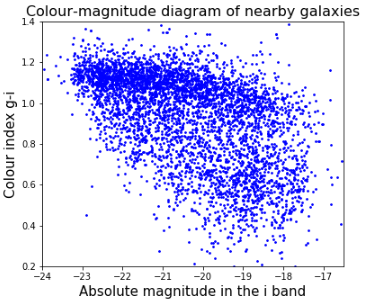
\includegraphics[width=\columnwidth]{images/CMDs/CMD-G_i-i.png}
    \caption[SDSS-IV MaNGA galaxy colour-magnitude diagram]{SDSS-IV MaNGA galaxy colour-magnitude diagram: the distribution of nearby galaxies from the Sloan Digital Sky Survey data release DR15. The colour index $g-i$ is plotted against i-band magnitude $M_i$. The distribution exhibits clear bimodality with late-type galaxies occupying a 'blue cloud' in the lower right while early-type galaxies form a 'red sequence' along the upper region of the diagram extending to brighter magnitudes. There is a clearly sparsely populated band separating the two densely populated regions, the so-called 'green valley'}
    \label{fig:CMD-G_i-i}
\end{figure}

\begin{figure}
    \centering
    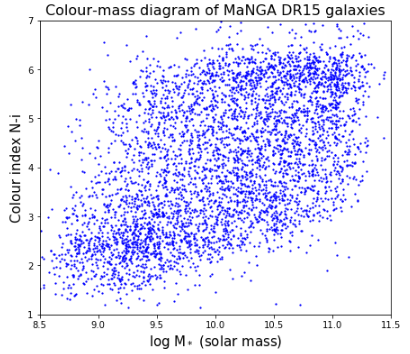
\includegraphics[width=\columnwidth]{images/CMDs/CMD-mass-1.png}
    \caption{An alternative representation of galaxy property distribution: colour index versus mass. The plot portrays the colour index near-UV - i band (NUV-i) versus log of stellar mass extracted from SDSS-IV MaNGA DR15 data. This representation of galaxy property distribution will be useful later.}
    \label{fig:CMD-mass-1}
\end{figure}

\subsection{Post starburst Galaxies}

Post-starburst (PSB) galaxies are a class of galaxies where the spectra indicate that star formation has ceased within the past gigayear or so. The is no spectral evidence of young O and B-type stars which will have gone supernova in the dynamical time since the starburst event. PSB spectra are dominated by the strong Balmer absorption lines H$\beta$, H$\gamma$, H$\delta$ indicative of a population of main sequence A- and F-type stars, particularly if a strong  H$\delta$ absorption line width is evident \citep{1997A&A...325.1025P}, while nebular emission lines characteristic of ongoing star formation, for example H$\alpha$ 6564 \AA\ and [OII] 3727\AA\, are weak or absent \citep{2001ApJ...547L..17B,2003PASJ...55..771G,2004MNRAS.355..713B,2005MNRAS.357..937G,2018MNRAS.477.1708P}. The morphology of PSBs is often that of early-type ellipticals and therefore PSBs are often referred to as E+A or K+A galaxies \citep{1983ApJ...270....7D,1996ApJ...466..104Z,2009ARA&A..47..159B}. These spectral observations are characteristic of a brief burst of star formation in the past 0.5 to 1.5 Gyr which has subsequently ceased, or been 'quenched' \citep{1983ApJ...270....7D,1987MNRAS.229..423C,1997A&A...325.1025P}. These spectral features are indicative that PSB galaxies are in transition on an evolutionary track from active star-forming galaxies to passive spheroids \citep{2004MNRAS.355..713B,2012MNRAS.420..672S,2013MNRAS.429.2212M}. Using a sample of a sample of low-redshift (z~0.1) E+A galaxies from the 2dF Galaxy Redshift Survey (2dFGRS) \citet{2004MNRAS.355..713B} find evidence of major mergers such as tidal tails and conclude that major mergers are an important formation mechanism for E+A PSB galaxies. A number of studies have shown that about half of galaxies have experienced recent rapid quenching while an evolutionary track to the red sequence \citep{Martin_2007,10.1111/j.1365-2966.2009.14537.x,2015MNRAS.450..435S}, however see \cite{2017ApJ...845..145W}. Quenching during mergers is also apparent in simulations, see e.g. \cite{2019MNRAS.484.2447D}.

In this study we analyse the kinematic properties of post-starburst galaxies to determine if there is evidence of major mergers in their kinematic signatures, and ask if major mergers could be the primary cause of the cessation of star formation. The objective would be to establish a link between merger activity, the quenching of star formation and morphological transition from blue late-type disc galaxies, through the green valley, to redder passive spheroids.

For this work we utilise a sample of 68 PSBs drawn from the SDSS-IV MaNGA (Mapping Nearby Galaxies at Apache Point Observatory integral field spectroscopic survey  as described in Section \ref{sec:data}.

[TODO: reformulate the following paragraph] See Vivienne's  papers researching PSBs: \citet{2017MNRAS.472.1401A} regarding the relationship of quenching and transition. \citet{2016MNRAS.463..832W} sets out the background work.

\subsection{Mergers and morphology}
\label{sec:mergers}

The term morphology refers to the structural features of galaxies. Commonly observed morphological features include discs, bulges, bars and spiral arms. These features form the basis of the Hubble classification system. A more complete classification system could also include other morphological features such as rings, warped discs, halos, tidal tails, arms and bridges. Studies of  morphological structure provides insights into galaxy evolution pathways. For a review of morphological types and their link to galaxy evolution see \cite{2011arXiv1102.0550B}.

Here we present a summary review of the literature on the detection of mergers and post-coalescence systems, or post-mergers, using observations of morphology. Mergers play a key role in galaxy evolution. In order to better understand the consequences of the merger process on evolution we need to employ refined methods to detect the morphological signatures of mergers. \cite{2016MNRAS.456.3032P} describe the morphological indicator designated 'shape asymmetry' for automated identification of galaxies exhibiting faint asymmetric tidal features indicative of ongoing or past mergers in order to determine whether PSBs play a transitory role in the buildup of the red sequence. \cite{2011arXiv1102.0550B} have developed numerical simulations to explore the sensitivity of galaxy mass ratio in the detection of major mergers in starburst galaxies. Adopting a similar but more extensive approach, \cite{2019ApJ...872...76N} developed a merger classification scheme that can be applied directly to SDSS images. Their method is based on hydrodynamical and N-body models of mergers, which were then trained on model SDSS images. They find their method is sensitive to mass ratio, and major mergers are also sensitive to asymmetry. In a progression of that earlier work  \cite{2019DDA....5020304N} have extended the SDSS image classification method to incorporate kinematic predictors derived from MaNGA stellar velocity maps. This is the first merger classification scheme that utilises both imaging and kinematics. The authors will apply the technique to explore how star formation rates change with different stages and types of merger. 

In this study, however, we are interested in the identification of past merger events, or post-mergers. Such major may have been the cause of star-formation quenching resulting in our transitional PSBs. The automated merger classification method of  \cite{2019DDA....5020304N} is expected to be of significant value in the context of identifying post-merger morphological features in the study PSB galaxies and their role in galaxy evolution. 


\subsection{kinematic position angle analysis}
Kinematic position angle analysis involves determining the major axes of the gas and stellar velocity fields. The method is employed in an effort to distinguish disc dominated systems from those that could indicate past major mergers. Commonly, gas and stellar velocity field (and their dispersion properties) are measured using \texttt{kinemetry} software package developed by \citet{2006MNRAS.366..787K}. Classification of a galaxy as a disc system or a merger depends on the relationship between the gas velocity $v$ and the gas velocity dispersion $\sigma$. Kinemetry can measure the kinematic position angle PA$_k$ of the major axes of the star velocity field and gas velocity field of a particular galaxy. The difference in the global position angles of the major axes of stellar and gas velocity field position angles yields the quantity $\Delta$PA$_k$ (measured in degrees). 

As an example of research work that applied kinemetry to the study of galaxy interaction the Calor Alto CALIFA survey \citet{2015A&A...582A..21B} studied a sample of 103 interacting galaxies at various merger stages: close companions, systems with evidence of morphological interaction and coalesced merger remnants. Classification of these systems was performed by measuring the difference in kinematic position angles of the stellar and ionised gas velocity fields. A sample of 80 non-interacting galaxies was used as a control sample. The findings reveals that 42\% of interacting galaxies have a misalignment of over 16\textdegree\ while this is evident in only 10\% of the control sample.

In a similarly motivated study \citet{2016A&A...591A..85B} examined the gas kinematics of nearby (ultra)luminous infrared galaxies ((U)LIRGs) at $z<0.1$. The objective was to analyse the kinematic properties of local (U)LIRGs and characterise their structures as those (U)LIRGs having disc structures (disc class), or displaying evidence of major merger activity (merger class). Their method employs optical integral field spectroscopy (IFS) data obtained at the VLT. H$\alpha$ emission is used as a gas velocity tracer. \citet{2016A&A...591A..85B} conclude that their results confirm that well-defined discs can be effectively distinguished from well-defined mergers but there is intermediate, indeterminate class. The authors note that the \texttt{kinemetry} method is sensitive to angular resolution of the integral field unit (IFU). Another example of the application of kinemetry is the earlier study conducted by \citet{2008ApJ...682..231S} which performed an  analysis of warm gas kinematics as traced by H$\alpha$ emission, but concentrating on sample at $z\sim2$ using the near IR IFS instrument SIMFONI on the VLT.

\subsection{Tilted ring fitting}
\label{sec:tilted-ring-fitting}

[TODO: write up some details of this method.]

The tilted ring fitting method enables kinematic features in disc galaxies, such as oval distortions and warped discs, to be quantified  \citep[see e.g.][]{1978PhDT.......195B,1981AJ.....86.1825B,2007A&A...468..731J}

\subsection{Radon transform analysis} 
Stellar and gas velocity fields that vary radially across the field can be analysed in detail using a technique employing the Radon transform. The method provides a greater level of detail, and thus some insight into the internal structures of galaxies than is possible with the kinematic position angle determination alone.


\subsection{Structure of the paper}
From this point onward the content of the paper is organised as follows: Details of the MaNGA survey and the selection criteria for our PSB sample and associated control galaxies are provided in Section \ref{sec:data}. Our main theme kinematic data analysis methods are presented in 2 sections: Section \ref{sec:methods-I-kinemetry} focusses on kinematic position angle analysis, while Section \ref{sec:methods-II-Radon} deals with the Radon transform method. Our research results from each of the methods are presented in Section \ref{sec:results}. Finally, a summary of the research and the conclusions drawn from this work, along with recommendations for further study are discussed in Section \ref{sec:discussion}.
